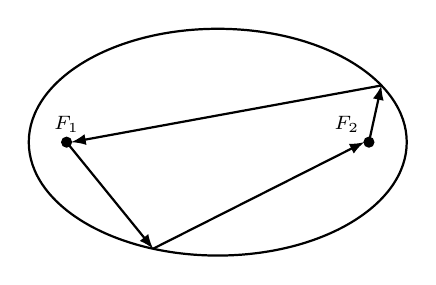
\begin{tikzpicture}[scale=1.2]%[width=\marginparwidth+25pt]

\draw [thick] (0,0) circle[x radius=2cm,y radius = 1.2cm];

\filldraw (1.6,0)  circle (1.5pt) node [above left] {\scriptsize $F_2$}
					(-1.6,0)  circle (1.5pt) node [above] {\scriptsize $F_1$};
					
\draw[->,>=latex,{\colorone},thick] (1.6,0) -- ({2*cos(30)},{1.2*sin(30)});% -- (-1.6,0);
\draw[->,>=latex,{\colorone},thick]({2*cos(30)},{1.2*sin(30)}) -- (-1.55,0);
\draw[->,>=latex,{\colortwo},thick] (-1.6,0) -- ({2*cos(250)},{1.2*sin(250)});% -- (-1.6,0);
\draw[->,>=latex,{\colortwo},thick]  ({2*cos(250)},{1.2*sin(250)}) -- (1.55,0);

\end{tikzpicture}
